\documentclass[12pt,english,a4paper]{article}

\usepackage[utf8]{inputenc}          % Allows UTF-8 encoded characters in the .tex-file.
\usepackage{babel,csquotes,textcomp} % Set LaTeX to structure the content following international academic standards.

% Include the TikZ-package for drawing figures.
%\usepackage{tikz}
%\usetikzlibrary{shapes.geometric,arrows}
%\usepackage{courier}

% Creates clickable hyperlinks in the PDF-document.
\usepackage{hyperref}
\usepackage{graphicx}
\usepackage{pdfpages}
\usepackage{listings}
\usepackage{wrapfig}
\usepackage{color}

\usepackage[
    backend=biber,
    style=alphabetic,
    sorting=ynt
]{biblatex}
\addbibresource{refs.bib}

\definecolor{mygreen}{rgb}{0,0.6,0}
\definecolor{mygray}{rgb}{0.5,0.5,0.5}
\definecolor{mymauve}{rgb}{0.58,0,0.82}

\lstset{ %
  basicstyle=\ttfamily\small,     
  backgroundcolor=\color{white},   % choose the background color
  breaklines=true,                 % automatic line breaking only at whitespace
  captionpos=b,                    % sets the caption-position to bottom
  commentstyle=\color{mygreen},    % comment style
  escapeinside={\%*}{*)},          % if you want to add LaTeX within your code
  keywordstyle=\color{blue},       % keyword style
  stringstyle=\color{mymauve},     % string literal style
}

\title{GPS Spoofing and the importance of correct time}
\author{Aril Johannes Schultzen}

\begin{document}
\maketitle
\thispagestyle{empty}
\setcounter{page}{0}
\newpage
\tableofcontents
\thispagestyle{empty}
\setcounter{page}{0}
\newpage
\thispagestyle{empty}
\setcounter{page}{0}

\begin{abstract}
Currently, this is not much more but comments and notes in order for me to write an essay, an essay meant for me to prepare for my work with my master thesis. This document does not represent the quality of the finished product in any way. Example cite \cite{KandR}
\end{abstract}

\newpage
\clearpage
\setcounter{page}{1}

\section{Global Positioning System: A short introduction}
In our everyday lives we are surrounded with GPS technology. In fields like emergency response, search and rescue, fleet management and even agriculture, it has become a vital tool of utmost importance to everyday operation. Satellite navigation in cars are more popular than ever and most phones are today sold with GPS receivers. The European Space Agency estimated that there were 2 billion GPS enabled devices by 2012 \cite{ESA}. What started out as a tool for the U.S military is now used by millions, if not billions of users all over the globe.

A common misconception is that the GPS satellites track \textit{you} in order to determine where you are. It actually works the other way around. You are, with your GPS receiver, tracking a set of satellites in order to establish your own position.The method used by your GPS receiver to determine its position is called \textit{trilateration}.Trilateration is used in geometry as a process of determining the location (absolute or relative) of point by measuring distance. It is often confused with triangulation which uses angles, where trilateration does not. At any given time, there are at least 24 GPS satellites orbiting the earth \cite{GPSGOV}. In order for a GPS receiver to determine its position, it will need 4 GPS satellites within line of sight \footnote{The line of sight requirement might seem unreasonable, but by the time the signal has reached earth, is has degraded to a minimum of -160 dBW \cite{NATINT}}. 
\begin{figure}[hb]
  \centering
  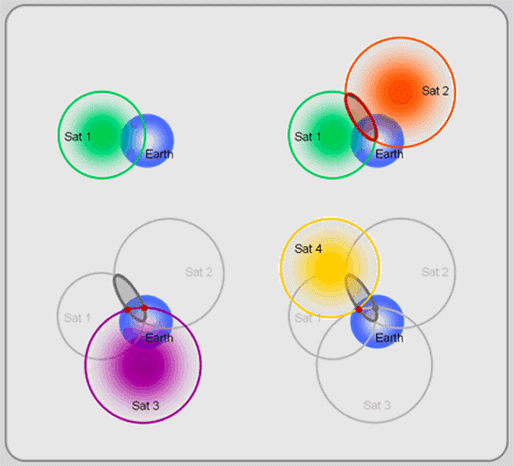
\includegraphics[scale=0.4]{trilaterate.jpg}
  \caption[GPS trilaterate figure]
   {Figure showing how GPS satellites are used to trilaterate to determine a GPS receivers position \cite{GISTRILATERATE}.}
\end{figure}

\section{Phasor Measurement Units}

\section{Signal interference}
\subsection{Locking on}
\subsection{Jamming}
\subsection{Spoofing}

By emitting a high-power signal at the GPS frequency, one can interfere with the signals emitted by the GPS satellites, effectively denying GPS receivers use of these signals. These signals are already weak considering their travel from space. Such an "attack", although effective, is pretty naive and easily recognized by the jammed party. After all, if you don't have a signal, you are probably being jammed. A more sophisticated approach is to emit a counterfeit signal in order to manipulate the receivers reported time or even position. IRAN, DRONE SPOOF STORY!. 

\subsection{Detection}
\subsection{Prevention}
\subsubsection{Encryption}

\section{Notes}
A way of detecting a clumsy attempt at jamming, would be to enter a "jam-mode" as soon as the location changes. The PMUs are not supposed to be moved. Why would they anyway? Moving power-plants? Discuss with Harald.

\newpage
\printbibliography[title={Complete Bibliography},heading=bibintoc]

\end{document}                    